
\documentclass[12pt]{article}
\usepackage{amsmath,amsthm,amssymb,amsfonts,fullpage,verbatim,bm,graphicx,enumerate,epstopdf,lscape,enumitem}
\usepackage[titletoc,title]{appendix}
\usepackage[dvipsnames,usenames]{color}
\usepackage[pdftex,pagebackref,colorlinks=true,pdfpagemode=UseNone,urlcolor=blue,linkcolor=blue,citecolor=BrickRed,pdfstartview=FitH,plainpages=true]{hyperref}
\usepackage[top=1.15in,bottom=1.15in,left=1.25in,right=1.25in,letterpaper]{geometry}
\usepackage[font=scriptsize]{caption}
\usepackage{cite}
\usepackage{caption,subcaption}
\usepackage{pbox}

\setlist{noitemsep}

\def\CC{\mathbb{C}}
\def\RR{\mathbb{R}}
\def\ZZ{\mathbb{Z}}
\def\PP{\mathbb{P}}
\def\EE{\mathbb{E}}

\newcommand{\Ga}{\alpha}
\newcommand{\Gb}{\beta}
\newcommand{\Gg}{\gamma}     \newcommand{\GG}{\Gamma}
\newcommand{\Gd}{\delta}     \newcommand{\GD}{\Delta}
\newcommand{\Ge}{\epsilon}
\newcommand{\Gf}{\phi}       \newcommand{\GF}{\Phi}
\newcommand{\Gh}{\theta}
\newcommand{\Gi}{\iota}
\newcommand{\Gk}{\kappa}
\newcommand{\Gl}{\lambda}    \newcommand{\GL}{\Lambda}
\newcommand{\Go}{\omega}     \newcommand{\GO}{\Omega}
\newcommand{\Gs}{\sigma}     \newcommand{\GS}{\Sigma}
\newcommand{\Gt}{\tau}
\newcommand{\Gz}{\zeta}
\newcommand{\s}{\sigma}
\newcommand{\tr}{\triangle}

\newcommand{\beginsupplement}{%
        \setcounter{table}{0}
        \renewcommand{\thetable}{S\arabic{table}}%
        \setcounter{figure}{0}
        \renewcommand{\thefigure}{S\arabic{figure}}%
     }

\begin{document}
\beginsupplement

\title{\textbf{Supplementary Materials}}
\date{}
\maketitle

\section{Simulation study for Gaussian data}
As noted in the main text, we performed an extensive simulation study for Gaussian errors using a variety of test functions (7 mean functions and 5 variance functions, including constant variance), signal-to-noise ratios (SNR = 1 and 3) and sample sizes ($T=256,512,1024$). For details of where the results are saved and what information they contain, refer to README.md from the \href{https://github.com/stephenslab/ashwave}{ashwave repo}. In particular, we include an RShiny app as an interactive way to present the results for $T=1024$, the code for which can be found in the \href{https://github.com/zrxing/dscr-smash}{dscr-smash repo}. For more details on the repo refer to the README.md file from the repo. In particular, users can view the boxplots of MISEs for the methods and test functions they are interested in by checking the appropriate boxes. For more details on the RShiny display refer to graphs.Rmd in the dscr-smash repo. For reference, the mean and variance functions used in the simulation studes are shown below in Figures \ref{gaus_mean} and \ref{gaus_var}.

\begin{figure}
\centering
    \begin{subfigure}[b]{0.48\textwidth}
        \centering
        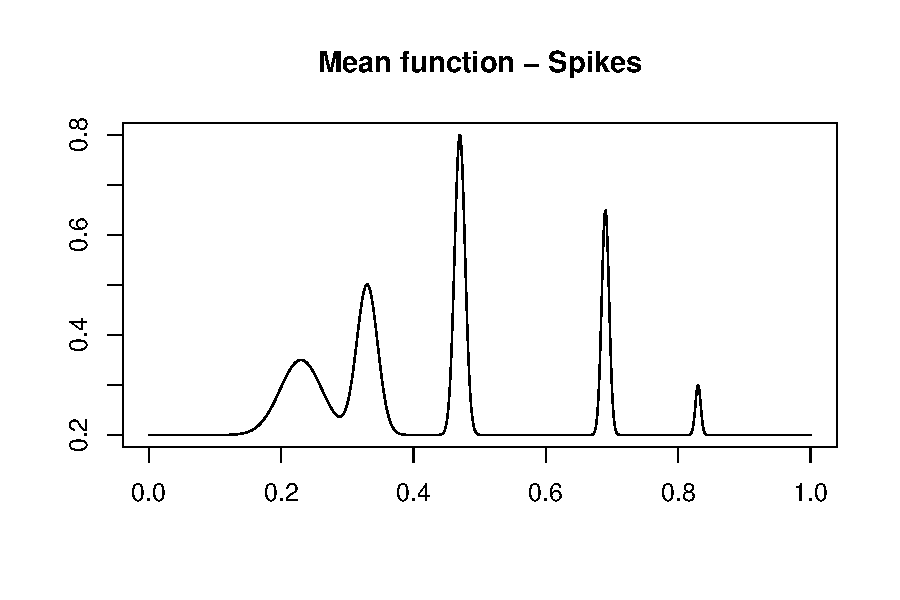
\includegraphics[width=\textwidth]{gaus_sp.pdf}
        \caption{}
        \label{fig:gaus_sp}
    \end{subfigure}
		\hfill
    \begin{subfigure}[b]{0.48\textwidth}
        \centering
        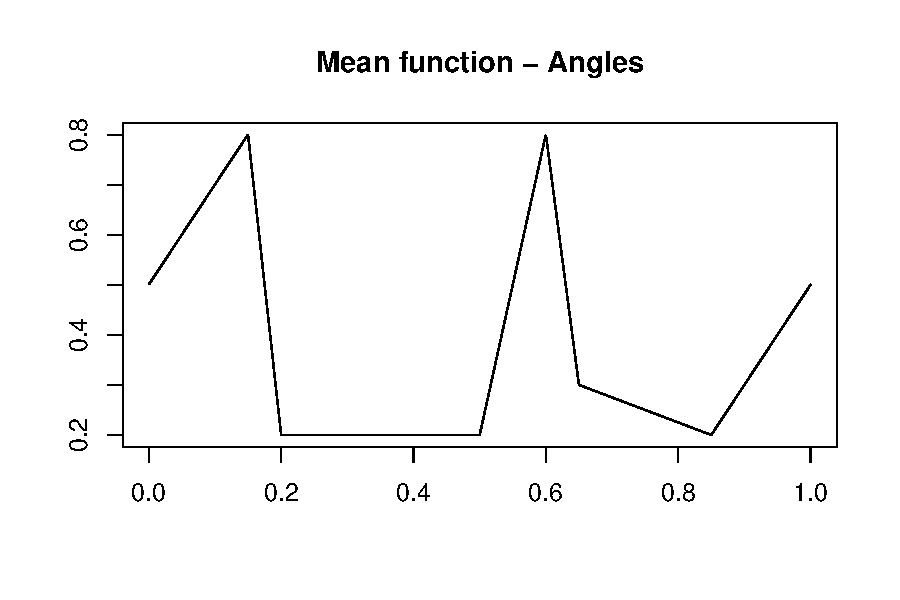
\includegraphics[width=\textwidth]{gaus_ang.pdf}
        \caption{}
        \label{fig:gaus_ang}
    \end{subfigure}
		\hfill
    \begin{subfigure}[b]{0.48\textwidth}
        \centering
        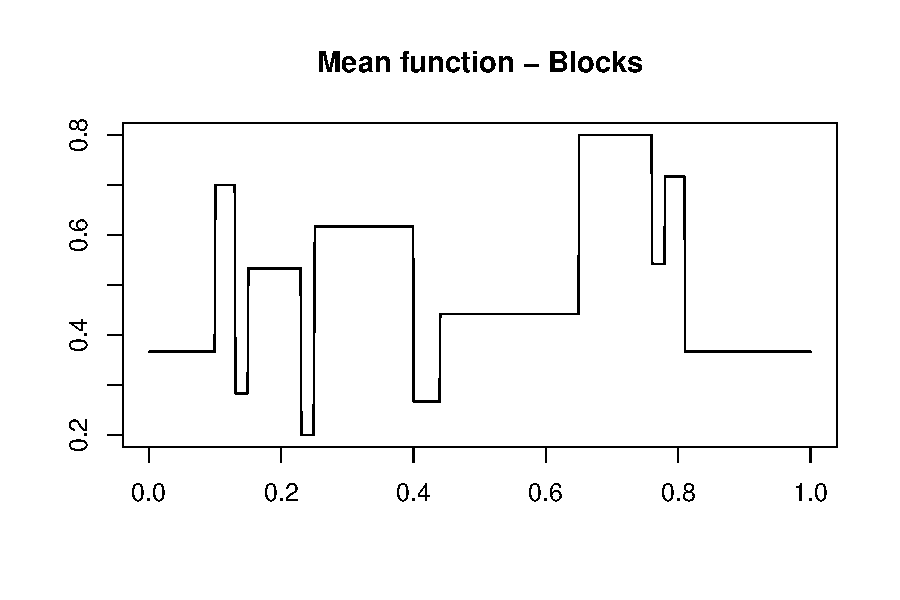
\includegraphics[width=\textwidth]{gaus_blk.pdf}
        \caption{}
        \label{fig:gaus_blk}
    \end{subfigure}
		\hfill
    \begin{subfigure}[b]{0.48\textwidth}
        \centering
        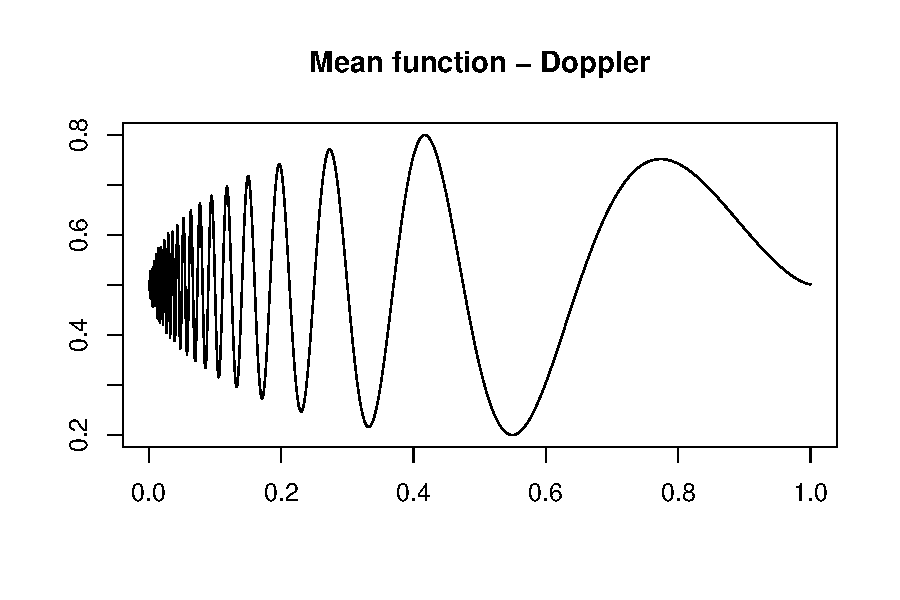
\includegraphics[width=\textwidth]{gaus_dop.pdf}
        \caption{}
        \label{fig:gaus_dop}
    \end{subfigure}
		\hfill
    \begin{subfigure}[b]{0.48\textwidth}
        \centering
        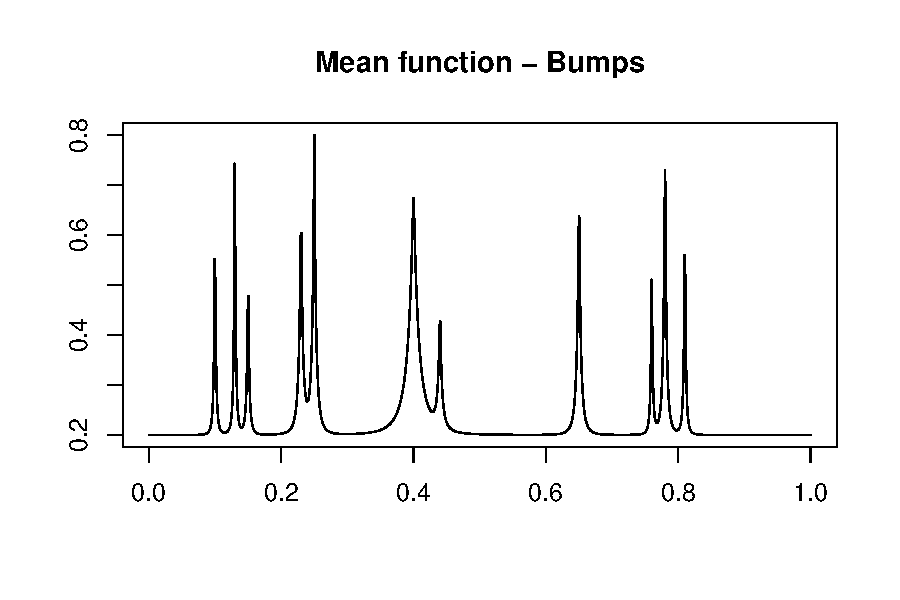
\includegraphics[width=\textwidth]{gaus_bump.pdf}
        \caption{}
        \label{fig:gaus_bump}
    \end{subfigure}
		\hfill
		\begin{subfigure}[b]{0.48\textwidth}
        \centering
        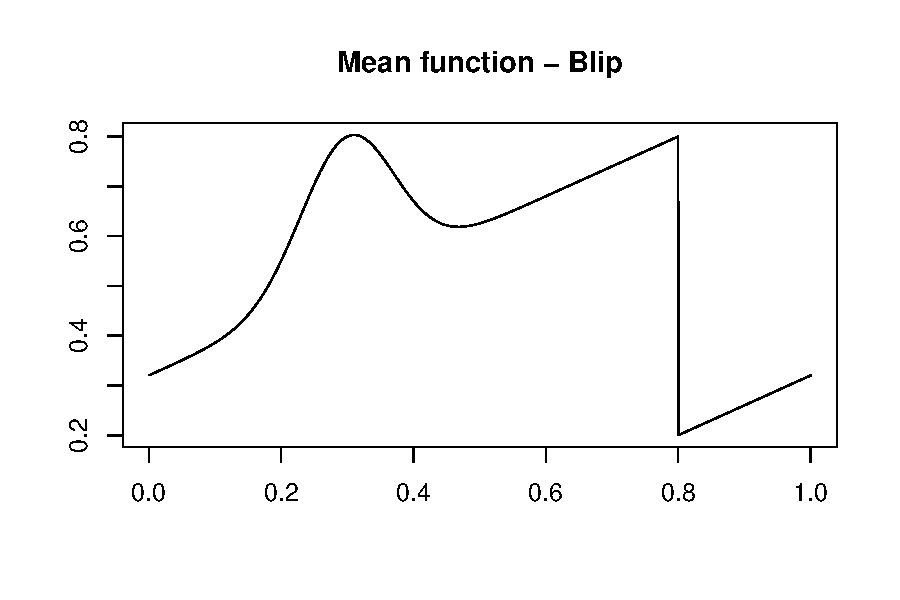
\includegraphics[width=\textwidth]{gaus_blip.pdf}
        \caption{}
        \label{fig:gaus_blip}
    \end{subfigure}
		\hfill
		\begin{subfigure}[b]{0.48\textwidth}
        \centering
        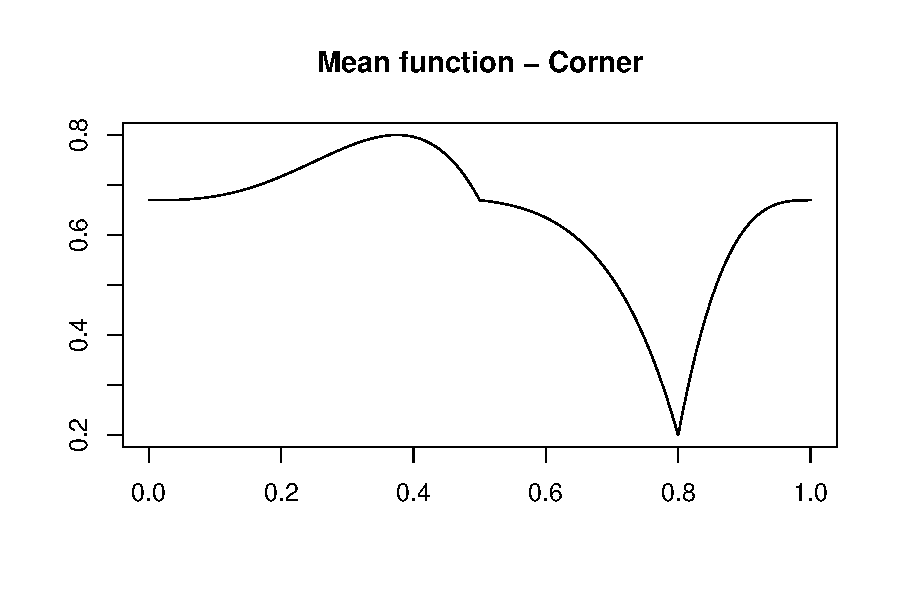
\includegraphics[width=\textwidth]{gaus_cor.pdf}
        \caption{}
        \label{fig:gaus_cor}
    \end{subfigure}
    \caption{The seven mean functions used in the Gaussian simulations, all scaled to be between 0.2 and 0.8.}
    \label{fig:gaus_mean}
\end{figure}


\begin{figure}
\centering
    \begin{subfigure}[b]{0.48\textwidth}
        \centering
        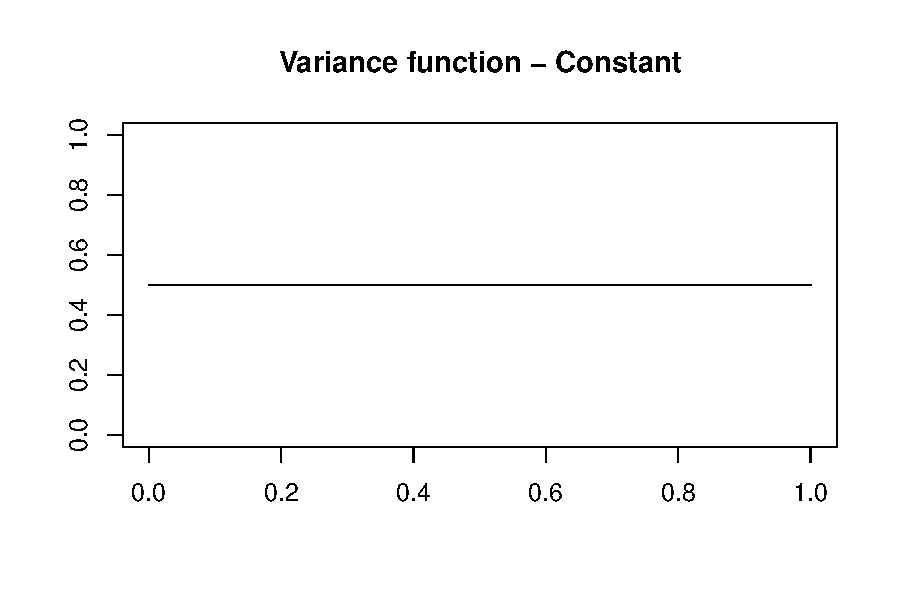
\includegraphics[width=\textwidth]{gaus_var_cons.pdf}
        \caption{}
        \label{fig:gaus_var_cons}
    \end{subfigure}
		\hfill
    \begin{subfigure}[b]{0.48\textwidth}
        \centering
        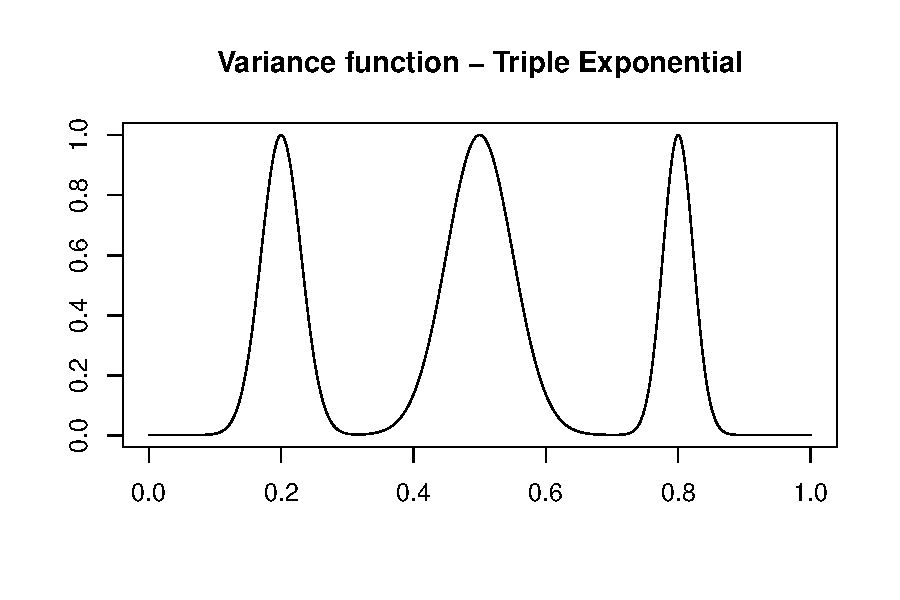
\includegraphics[width=\textwidth]{gaus_var_texp.pdf}
        \caption{}
        \label{fig:gaus_var_texp}
    \end{subfigure}
		\hfill
    \begin{subfigure}[b]{0.48\textwidth}
        \centering
        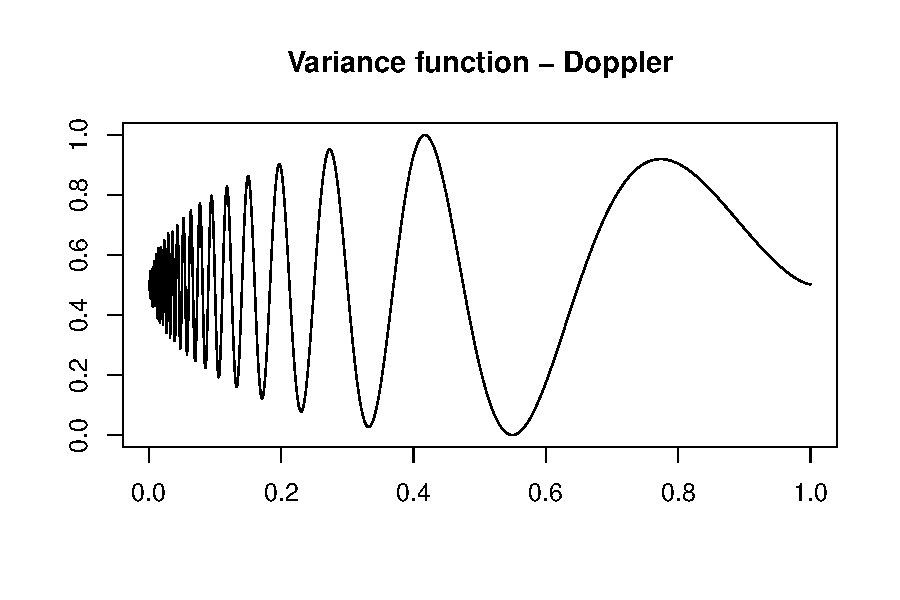
\includegraphics[width=\textwidth]{gaus_var_dop.pdf}
        \caption{}
        \label{fig:gaus_var_dop}
    \end{subfigure}
		\hfill
    \begin{subfigure}[b]{0.48\textwidth}
        \centering
        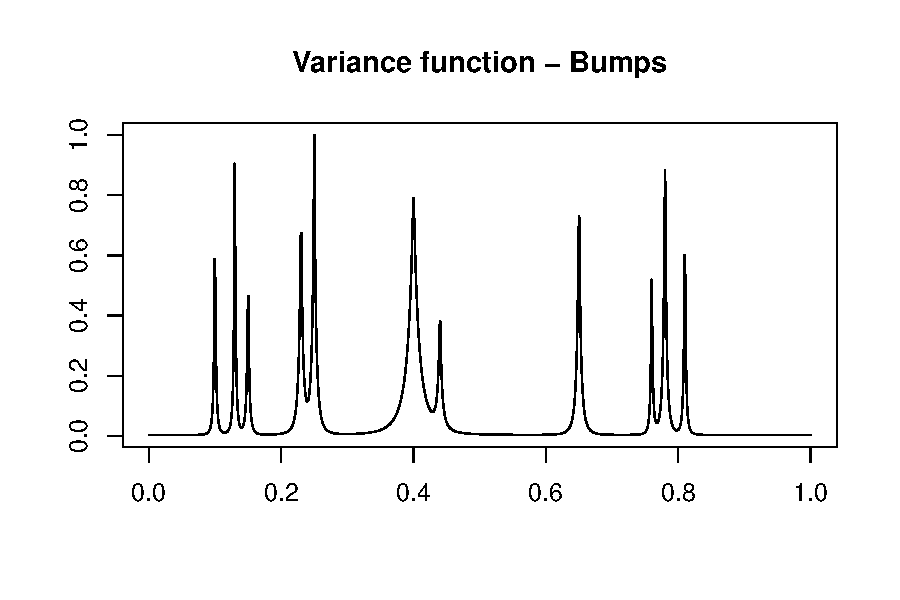
\includegraphics[width=\textwidth]{gaus_var_bump.pdf}
        \caption{}
        \label{fig:gaus_var_bump}
    \end{subfigure}
		\hfill
    \begin{subfigure}[b]{0.48\textwidth}
        \centering
        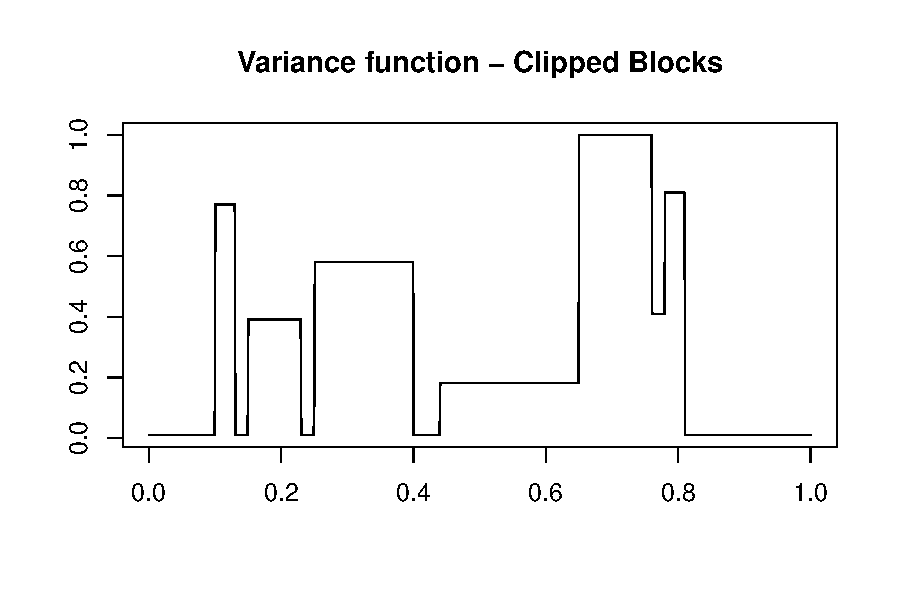
\includegraphics[width=\textwidth]{gaus_var_cblk.pdf}
        \caption{}
        \label{fig:gaus_var_cblk}
    \end{subfigure}
    \caption{The five variance functions used in the Gaussian simulations, which are rescaled in the simulations to achieve the desired signal to noise ratios.}
    \label{fig:gaus_var}
\end{figure}


In addition to the performance of the various methods, we also provide code in the \href{https://github.com/stephenslab/ashwave}{ashwave repo} generating a table that provide additional details for each method used, including the associated software, variance assumption, wavelet basis, shrinkage procedure used, and other relevant information.


\section{Simulation study for Poisson data}
The results from the simulation study for Poisson noise are shown in the following tables. For reference, we first plot the intensity functions used in the simulation studies in Figure \ref{fig:pois_mean}. Each of the six tables (\ref{table:pois_sp}-\ref{table:pois_b}) presents results for the corresponding mean function, and includes results for all three (min,max) intensity levels ((0.01,3), (1/8,8), (1/128,128)). As mentioned in the main text, we also explored several options for the Gaussian de-noising stage of the HF algorithm, and include the results in the following tables. Specifically, we considered four different options (all with 50 external cyclespins):
\begin{enumerate}
\item Hybrid of (1) Greedy tree de-noising (\cite{Baraniuk1999Optimal}) and (2) wavelet thresholding using ``leave-half-out'' crossvalidation (eg \cite{Nason1995Choice}). $j_0=3$ (default), and the noise level was estimated from the data. This corresponds to \textbf{H:CV+BT CS} in \cite{Fryzlewicz2004HaarFisz}. Note that the algorithm does not always converge for this option, resulting in NA values in the tables below.
\item Wavelet thresholding using the universal threshold (\cite{Donoho1994Ideal}). $j_0=3$ (default), and the noise level was estimated from the data. This corresponds to \textbf{F$\bowtie$U CS} in \cite{Fryzlewicz2004HaarFisz}.
\item Wavelet thresholding using the universal threshold for the non-decimated wavelet transform. Results averaged over $j_0=4,5,6,7$, and the noise level was estimated from the data.
\item Wavelet thresholding using the universal threshold for the non-decimated wavelet transform. Results average over $j_0=4,5,6,7$, and the noise level was set to be 1 (which is the asymptotic variance under the Fisz transform). This is the option for which we included the results in the main text, as it had the best overall performance.
\end{enumerate}


\begin{figure}
\centering
    \begin{subfigure}[b]{0.48\textwidth}
        \centering
        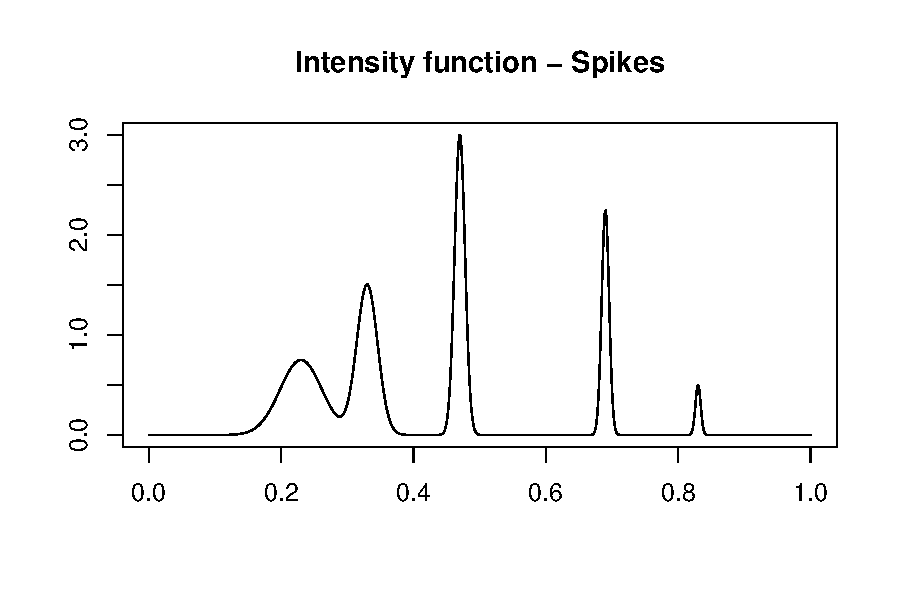
\includegraphics[width=\textwidth]{pois_sp.pdf}
        \caption{}
        \label{fig:pois_sp}
    \end{subfigure}
		\hfill
    \begin{subfigure}[b]{0.48\textwidth}
        \centering
        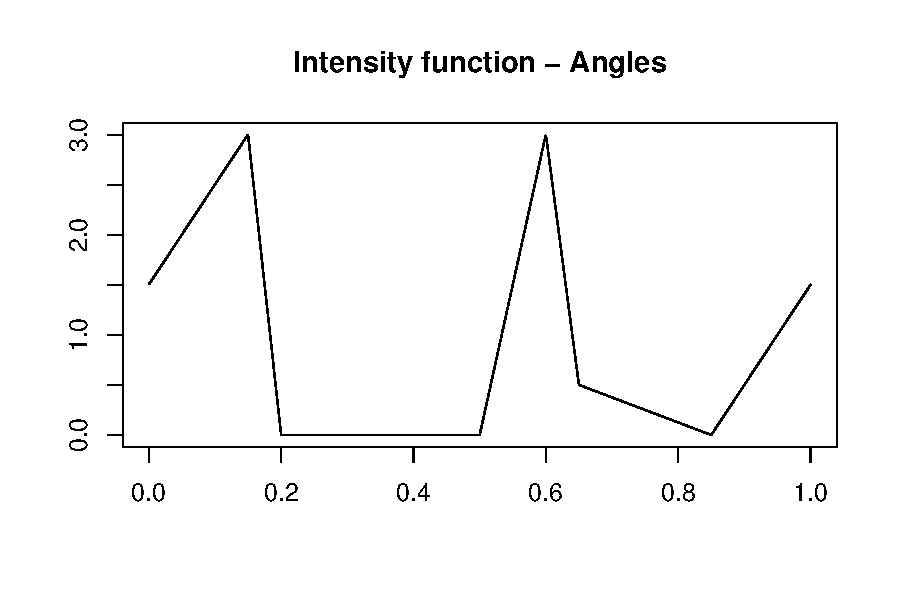
\includegraphics[width=\textwidth]{pois_ang.pdf}
        \caption{}
        \label{fig:pois_ang}
    \end{subfigure}
		\hfill
    \begin{subfigure}[b]{0.48\textwidth}
        \centering
        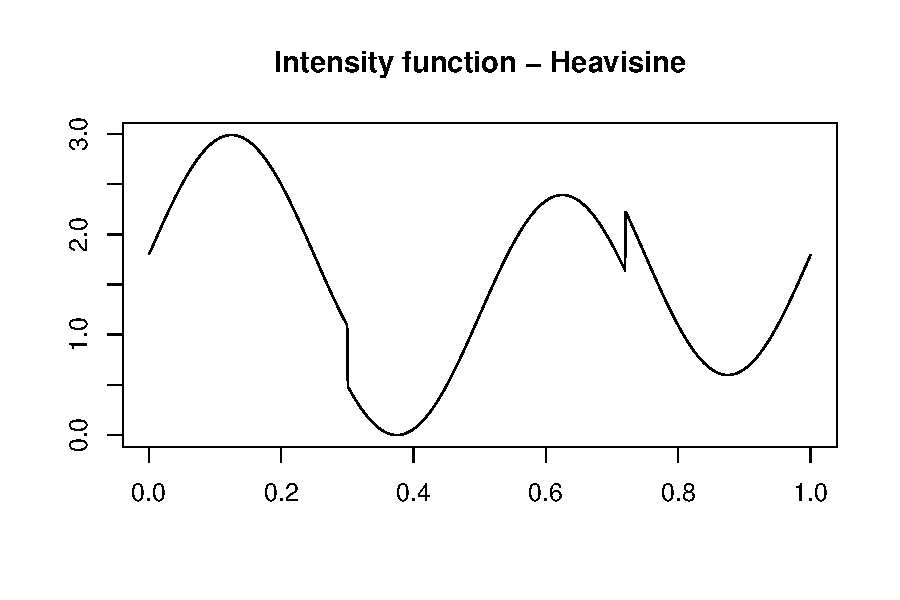
\includegraphics[width=\textwidth]{pois_hs.pdf}
        \caption{}
        \label{fig:pois_hs}
    \end{subfigure}
		\hfill
    \begin{subfigure}[b]{0.48\textwidth}
        \centering
        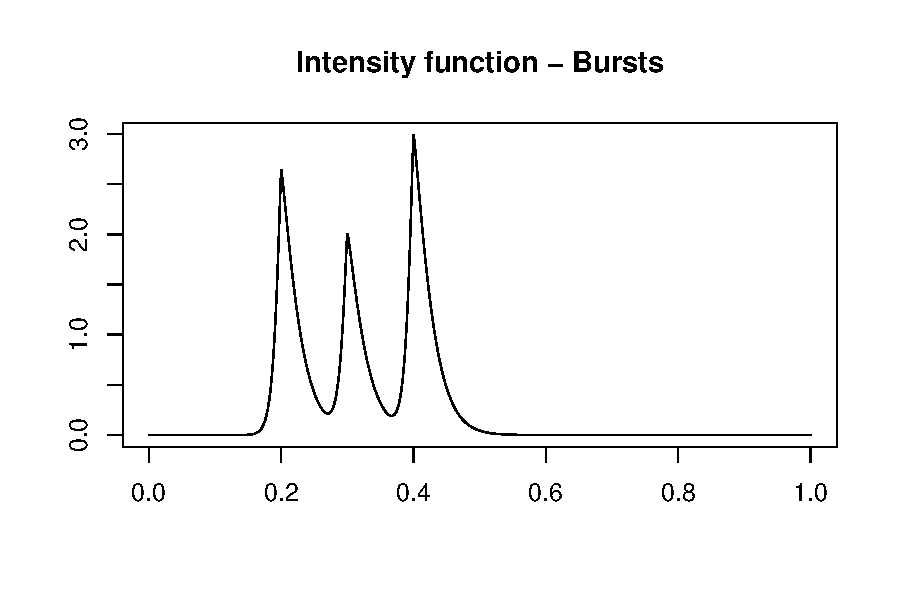
\includegraphics[width=\textwidth]{pois_bur.pdf}
        \caption{}
        \label{fig:pois_bur}
    \end{subfigure}
		\hfill
    \begin{subfigure}[b]{0.48\textwidth}
        \centering
        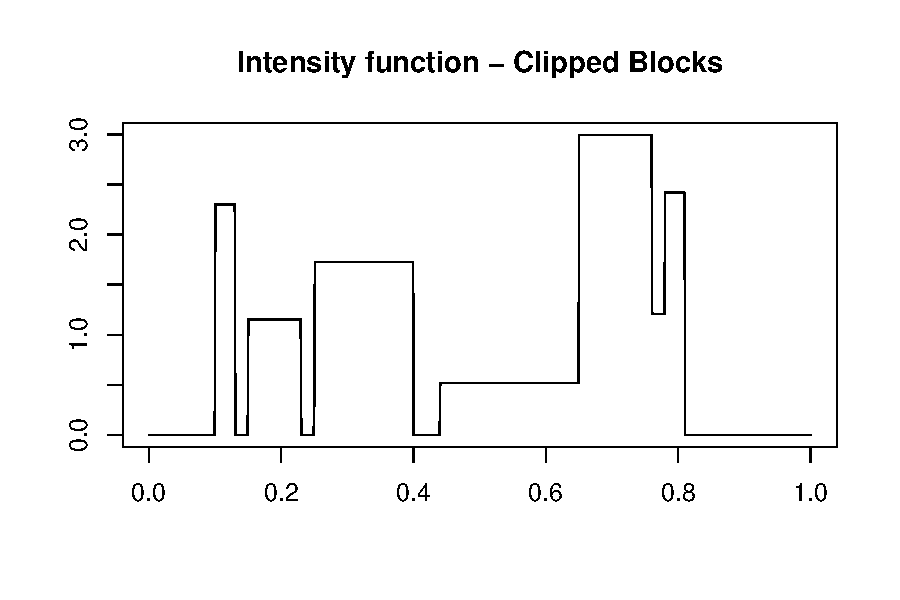
\includegraphics[width=\textwidth]{pois_cblk.pdf}
        \caption{}
        \label{fig:pois_cblk}
    \end{subfigure}
		\hfill
		\begin{subfigure}[b]{0.48\textwidth}
        \centering
        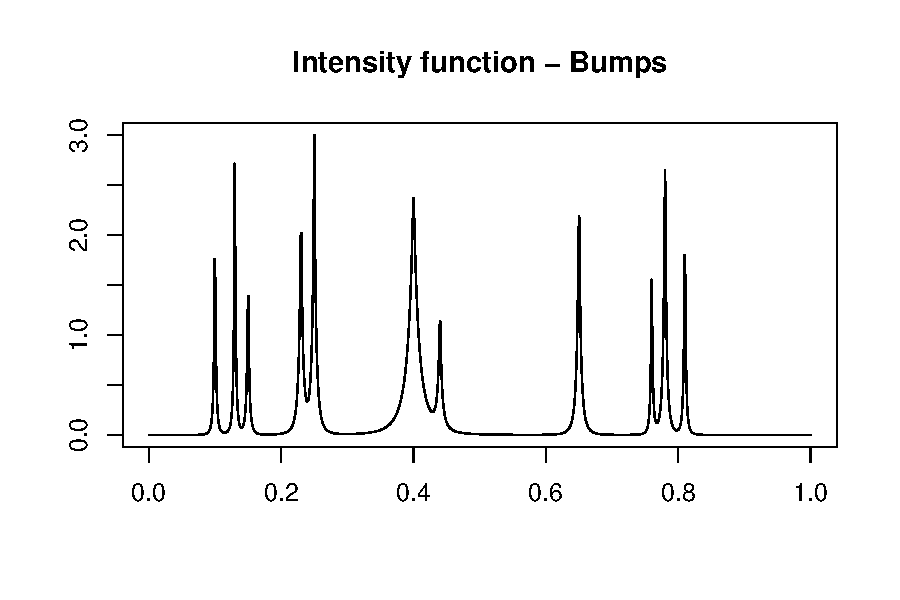
\includegraphics[width=\textwidth]{pois_bump.pdf}
        \caption{}
        \label{fig:pois_bump}
    \end{subfigure}
    \caption{The six intensity functions used in the Poisson simulations, which are rescaled to achieve the desired (min,max) intensities in the simulations.}
    \label{fig:pois_mean}
\end{figure}

\begin{table}[ht]
\centering
\begin{tabular}{rrrr}
  \hline
 & (0.01,3) & (1/8,8) & (1/128,128) \\ 
  \hline
SMASH & \textcolor{red}{690.01} & 329.26 & 48.87 \\ 
  BMSM & 1007.34 & 397.79 & 41.88 \\ 
  BMMIM & 930.08 & 436.54 & 368.36 \\ 
	Haar-Fisz (1) & 8194.60 & NA & 184.81 \\
	Haar-Fisz (2) & 8074.05 & 408.32 & 158.68 \\
	Haar-Fisz (3) & 5904.98 & 317.12 & 73.00 \\	
  Haar-Fisz (4) & 722.19 & \textcolor{red}{287.44} & \textcolor{red}{18.06} \\ 
  Anscombe & 1329.87 & 388.59 & 18.17 \\ 
  Haar thresholds & 803.89 & 326.11 & 120.02 \\ 
  L1\_penalty & 3085.65 & 2209.67 & 1516.78 \\ 
   \hline
\end{tabular}
\caption{Comparison of methods for denoising Poisson data for the ``Spikes'' test function for 3 different (min,max) intensities ((0.01,3), (1/8,8), (1/128,128)). Performance is measured using MISE over 100 independent datasets, with smaller values indicating better performance. Values colored in red indicates the smallest MISE amongst all methods (excluding Haar-Fisz (1-3)) for a given (min, max) intensity.} 
\label{table:pois_sp}
\end{table}


\begin{table}[ht]
\centering
\begin{tabular}{rrrr}
  \hline
 & (0.01,3) & (1/8,8) & (1/128,128) \\ 
  \hline
SMASH & \textcolor{red}{145.26} & \textcolor{red}{68.47} & 10.25 \\ 
  BMSM & 147.40 & 73.87 & 10.49 \\ 
  BMMIM & 245.89 & 100.17 & 71.26 \\ 
	Haar-Fisz (1) & NA & 91.86 & 25.23 \\
	Haar-Fisz (2) & 1020.76 & 78.84 & 12.22 \\
	Haar-Fisz (3) & 614.95 & 125.78 & 11.29 \\	
  Haar-Fisz (4) & 314.41 & 122.79 & \textcolor{red}{9.08} \\ 
  Anscombe & 419.04 & 146.64 & 9.50 \\ 
  Haar thresholds & 264.38 & 162.16 & 89.37 \\ 
  L1\_penalty & 655.82 & 284.75 & 2979.23 \\ 
   \hline
\end{tabular}
\caption{Comparison of methods for denoising Poisson data for the ``Angles'' test function for 3 different (min,max) intensities ((0.01,3), (1/8,8), (1/128,128)). Performance is measured using MISE over 100 independent datasets, with smaller values indicating better performance. Values colored in red indicates the smallest MISE amongst all methods (excluding Haar-Fisz (1-3)) for a given (min, max) intensity.} 
\label{table:pois_ang}
\end{table}

\begin{table}[ht]
\centering
\begin{tabular}{rrrr}
  \hline
 & (0.01,3) & (1/8,8) & (1/128,128) \\ 
  \hline
SMASH & \textcolor{red}{81.41} & \textcolor{red}{43.21} & \textcolor{red}{7.21} \\ 
  BMSM & 85.29 & 44.22 & 7.35 \\ 
  BMMIM & 205.09 & 81.49 & 11.22 \\ 
	Haar-Fisz (1) & 135.42 & 62.01 & 8.10 \\
	Haar-Fisz (2) & 105.72 & 61.66 & 6.29 \\
	Haar-Fisz (3) & 273.97 & 104.99 & 9.98 \\	
	Haar-Fisz (4) & 274.26 & 105.47 & 9.23 \\ 
  Anscombe & 372.06 & 128.43 & 9.10 \\ 
  Haar thresholds & 226.27 & 143.01 & 85.74 \\ 
  L1\_penalty & 385.47 & 71.17 & 8.68 \\ 
   \hline
\end{tabular}
\caption{Comparison of methods for denoising Poisson data for the ``Heavisine'' test function for 3 different (min,max) intensities ((0.01,3), (1/8,8), (1/128,128)). Performance is measured using MISE over 100 independent datasets, with smaller values indicating better performance. Values colored in red indicates the smallest MISE amongst all methods (excluding Haar-Fisz (1-3)) for a given (min, max) intensity.} 
\label{table:pois_hs}
\end{table}

\begin{table}[ht]
\centering
\begin{tabular}{rrrr}
  \hline
 & (0.01,3) & (1/8,8) & (1/128,128) \\ 
  \hline
SMASH & \textcolor{red}{487.34} & \textcolor{red}{234.35} & 33.11 \\ 
  BMSM & 706.04 & 301.86 & 34.42 \\ 
  BMMIM & 654.11 & 290.91 & 531.79 \\ 
	Haar-Fisz (1) & 6870.35 & NA & 157.15 \\
	Haar-Fisz (2) & 6807.29 & 384.56 & 149.23 \\
	Haar-Fisz (3) & 5619.13 & 318.57 & 94.20 \\	
	Haar-Fisz (4) & 618.39 & 299.39 & \textcolor{red}{25.20} \\ 
  Anscombe & 869.16 & 343.15 & 26.03 \\ 
  Haar thresholds & 540.58 & 271.16 & 107.44 \\ 
  L1\_penalty & 1836.73 & 1280.16 & 719.59 \\ 
   \hline
\end{tabular}
\caption{Comparison of methods for denoising Poisson data for the ``Bursts'' test function for 3 different (min,max) intensities ((0.01,3), (1/8,8), (1/128,128)). Performance is measured using MISE over 100 independent datasets, with smaller values indicating better performance. Values colored in red indicates the smallest MISE amongst all methods (excluding Haar-Fisz (1-3)) for a given (min, max) intensity.} 
\label{table:pois_bur}
\end{table}

\begin{table}[ht]
\centering
\begin{tabular}{rrrr}
  \hline
 & (0.01,3) & (1/8,8) & (1/128,128) \\ 
  \hline
SMASH & \textcolor{red}{307.80} & \textcolor{red}{137.28} & \textcolor{red}{6.82} \\ 
  BMSM & 355.15 & 143.09 & 6.91 \\ 
  BMMIM & 472.24 & 205.20 & 150.03 \\ 
	Haar-Fisz (1) & NA & 141.71 & 31.23 \\
	Haar-Fisz (2) & 879.20 & 316.44 & 26.71 \\
	Haar-Fisz (3) & 741.49 & 389.79 & 48.41 \\	
	Haar-Fisz (4) & 632.21 & 338.55 & 29.72 \\ 
  Anscombe & 804.70 & 384.46 & 28.94 \\ 
  Haar thresholds & 467.64 & 228.14 & 82.99 \\ 
  L1\_penalty & 1021.58 & 627.67 & 1961.42 \\ 
   \hline
\end{tabular}
\caption{Comparison of methods for denoising Poisson data for the ``Clipped Blocks'' test function for 3 different (min,max) intensities ((0.01,3), (1/8,8), (1/128,128)). Performance is measured using MISE over 100 independent datasets, with smaller values indicating better performance. Values colored in red indicates the smallest MISE amongst all methods (excluding Haar-Fisz (1-3)) for a given (min, max) intensity.} 
\label{table:pois_cb}
\end{table}

\begin{table}[ht]
\centering
\begin{tabular}{rrrr}
  \hline
 & (0.01,3) & (1/8,8) & (1/128,128) \\ 
  \hline
SMASH & \textcolor{red}{2597.46} & \textcolor{red}{1194.62} & \textcolor{red}{141.21} \\ 
  BMSM & 4036.77 & 1889.94 & 171.07 \\ 
  BMMIM & 3440.75 & 2226.20 & 291.22 \\ 
	Haar-Fisz (1) & 9515.68 & NA & 187.6 \\
	Haar-Fisz (2) & 9249.05 & 1288.30 & 130.19 \\
	Haar-Fisz (3) & 6286.05 & 1756.08 & 248.28 \\	
	Haar-Fisz (4) & 3113.37 & 1658.74 & 184.66 \\ 
  Anscombe & 4038.42 & 2241.74 & 195.75 \\ 
  Haar thresholds & 3517.89 & 1652.55 & 173.72 \\ 
  L1\_penalty & 4705.77 & 3676.42 & 1774.51 \\ 
   \hline
\end{tabular}
\caption{Comparison of methods for denoising Poisson data for the ``Bumps'' test function for 3 different (min,max) intensities ((0.01,3), (1/8,8), (1/128,128)). Performance is measured using MISE over 100 independent datasets, with smaller values indicating better performance. Values colored in red indicates the smallest MISE amongst all methods (excluding Haar-Fisz (1-3)) for a given (min, max) intensity.} 
\label{table:pois_b}
\end{table}





%
%In addition we explore the results from trying out different Gaussian de-noising procedures for the second step of the Haar-Fisz (HF) algorithm.
%
%\begin{table}[ht]
%\centering
%\begin{tabular}{lrrrr}
  %\hline
 %& BT + CV & \pbox{20cm}{TI-universal \\ sd = 1} & \pbox{20cm}{TI-universal \\ sd estimated} & \pbox{20cm}{Universal \\ thresholding} \\ 
  %\hline
%j0 = 4 \\
 %(where applicable) & NA & 280.29 & 312.35 & 408.32 \\ 
  %j0 = 5 \\
 %(where applicable) & NA & 246.95 & 234.90 & 408.32 \\ 
  %j0 = 6 \\
 %(where applicable) & NA & 254.54 & 261.18 & 408.32 \\ 
  %j0 = 7 \\
 %(where applicable) & NA & 367.98 & 460.04 & 408.32 \\ 
  %Average \\
 %(where applicable) & NA & 287.44 & 317.12 & 408.32 \\ 
   %\hline
%\end{tabular}
%\caption{Comparison of different options for HF for the ``Spikes'' test function for (min,max) intensity = (1/8,8). Options BT + CV and Universal thresholding correspond to the two default oness used in {Fryzlewicz2004HaarFisz}, with primary resolution j0 =3. TI-universal corresponds to universal thresholding with translational invariance, with sd either estimated from the data or set to be 1 (which is the asymptotic variance). For TI-universal, we ran the HF with j0 = 4, 5, 6 and 7, corresponding to the first 4 rows, as well as the average of all 4 values, corresponding to the 5th row. Note here that BT + CV do not converge due to numerical issues. Performance is measured using MISE over 100 independent datasets, with smaller values indicating better performance.} 
%\label{table:pois_hf_sp_8}
%\end{table}
%
%
%\begin{table}[ht]
%\centering
%\begin{tabular}{lrrrr}
  %\hline
 %& BT + CV & \pbox{20cm}{TI-universal \\ sd = 1} & \pbox{20cm}{TI-universal \\ sd estimated} & \pbox{20cm}{Universal \\ thresholding} \\ 
  %\hline
%j0 = 4 \\
 %(where applicable) & 91.86 & 70.11 & 77.37 & 78.84 \\ 
  %j0 = 5 \\
 %(where applicable) & 91.86 & 65.09 & 65.43 & 78.84 \\ 
  %j0 = 6 \\
 %(where applicable) & 91.86 & 121.87 & 123.01 & 78.84 \\ 
  %j0 = 7 \\
 %(where applicable) & 91.86 & 234.08 & 237.28 & 78.84 \\ 
  %Average \\
 %(where applicable) & 91.86 & 122.79 & 125.77 & 78.84 \\ 
   %\hline
%\end{tabular}
%\caption{Comparison of different options for HF for the ``Angles'' test function for (min,max) intensity = (1/8,8). Options BT + CV and Universal thresholding correspond to the two default oness used in {Fryzlewicz2004HaarFisz}, with primary resolution j0 =3. TI-universal corresponds to universal thresholding with translational invariance, with sd either estimated from the data or set to be 1 (which is the asymptotic variance). For TI-universal, we ran the HF with j0 = 4, 5, 6 and 7, corresponding to the first 4 rows, as well as the average of all 4 values, corresponding to the 5th row. Performance is measured using MISE over 100 independent datasets, with smaller values indicating better performance.} 
%\label{table:pois_hf_ang_8}
%\end{table}
%
%
%\begin{table}[ht]
%\centering
%\begin{tabular}{lrrrr}
  %\hline
 %& BT + CV & \pbox{20cm}{TI-universal \\ sd = 1} & \pbox{20cm}{TI-universal \\ sd estimated} & \pbox{20cm}{Universal \\ thresholding} \\ 
  %\hline
%j0 = 4 \\
 %(where applicable) & 62.01 & 38.51 & 37.96 & 61.66 \\ 
  %j0 = 5 \\
 %(where applicable) & 62.01 & 59.24 & 58.61 & 61.66 \\ 
  %j0 = 6 \\
 %(where applicable) & 62.01 & 110.77 & 110.22 & 61.66 \\ 
  %j0 = 7 \\
 %(where applicable) & 62.01 & 213.36 & 213.13 & 61.66 \\ 
  %Average \\
 %(where applicable) & 62.01 & 105.47 & 104.98 & 61.66 \\ 
   %\hline
%\end{tabular}
%\caption{Comparison of different options for HF for the ``Heavisine'' test function for (min,max) intensity = (1/8,8). Options BT + CV and Universal thresholding correspond to the two default oness used in {Fryzlewicz2004HaarFisz}, with primary resolution j0 =3. TI-universal corresponds to universal thresholding with translational invariance, with sd either estimated from the data or set to be 1 (which is the asymptotic variance). For TI-universal, we ran the HF with j0 = 4, 5, 6 and 7, corresponding to the first 4 rows, as well as the average of all 4 values, corresponding to the 5th row. Performance is measured using MISE over 100 independent datasets, with smaller values indicating better performance.} 
%\label{table:pois_hf_hs_8}
%\end{table}
%
%\begin{table}[ht]
%\centering
%\begin{tabular}{lrrrr}
  %\hline
 %& BT + CV & \pbox{20cm}{TI-universal \\ sd = 1} & \pbox{20cm}{TI-universal \\ sd estimated} & \pbox{20cm}{Universal \\ thresholding} \\ 
  %\hline
%j0 = 4 \\
 %(where applicable) & NA & 331.11 & 340.45 & 384.56 \\ 
  %j0 = 5 \\
 %(where applicable) & NA & 323.51 & 294.31 & 384.56 \\ 
  %j0 = 6 \\
 %(where applicable) & NA & 211.35 & 235.24 & 384.56 \\ 
  %j0 = 7 \\
 %(where applicable) & NA & 331.58 & 404.25 & 384.56 \\ 
  %Average \\
 %(where applicable) & NA & 299.39 & 318.56 & 384.56 \\ 
   %\hline
%\end{tabular}
%\caption{Comparison of different options for HF for the ``Bursts'' test function for (min,max) intensity = (1/8,8). Options BT + CV and Universal thresholding correspond to the two default oness used in {Fryzlewicz2004HaarFisz}, with primary resolution j0 =3. TI-universal corresponds to universal thresholding with translational invariance, with sd either estimated from the data or set to be 1 (which is the asymptotic variance). For TI-universal, we ran the HF with j0 = 4, 5, 6 and 7, corresponding to the first 4 rows, as well as the average of all 4 values, corresponding to the 5th row. Note here that BT + CV do not converge due to numerical issues. Performance is measured using MISE over 100 independent datasets, with smaller values indicating better performance.} 
%\label{table:pois_hf_bur_8}
%\end{table}
%
%
%\begin{table}[ht]
%\centering
%\begin{tabular}{lrrrr}
  %\hline
 %& BT + CV & \pbox{20cm}{TI-universal \\ sd = 1} & \pbox{20cm}{TI-universal \\ sd estimated} & \pbox{20cm}{Universal \\ thresholding} \\ 
  %\hline
%j0 = 4 \\
 %(where applicable) & 141.71 & 337.24 & 486.16 & 316.44 \\ 
  %j0 = 5 \\
 %(where applicable) & 141.71 & 333.16 & 384.27 & 316.44 \\ 
  %j0 = 6 \\
 %(where applicable) & 141.71 & 341.66 & 346.94 & 316.44 \\ 
  %j0 = 7 \\
 %(where applicable) & 141.71 & 342.12 & 341.76 & 316.44 \\ 
  %Average \\
 %(where applicable) & 141.71 & 338.54 & 389.78 & 316.44 \\ 
   %\hline
%\end{tabular}
%\caption{Comparison of different options for HF for the ``Clipped Blocks'' test function for (min,max) intensity = (1/8,8). Options BT + CV and Universal thresholding correspond to the two default oness used in {Fryzlewicz2004HaarFisz}, with primary resolution j0 =3. TI-universal corresponds to universal thresholding with translational invariance, with sd either estimated from the data or set to be 1 (which is the asymptotic variance). For TI-universal, we ran the HF with j0 = 4, 5, 6 and 7, corresponding to the first 4 rows, as well as the average of all 4 values, corresponding to the 5th row. Performance is measured using MISE over 100 independent datasets, with smaller values indicating better performance.} 
%\label{table:pois_hf_cb_8}
%\end{table}
%
%\begin{table}[ht]
%\centering
%\begin{tabular}{lrrrr}
  %\hline
 %& BT + CV & \pbox{20cm}{TI-universal \\ sd = 1} & \pbox{20cm}{TI-universal \\ sd estimated} & \pbox{20cm}{Universal \\ thresholding} \\ 
  %\hline
%j0 = 4 \\
 %(where applicable) & NA & 1918.04 & 2553.46 & 1288.30 \\ 
  %j0 = 5 \\
 %(where applicable) & NA & 1815.30 & 1853.65 & 1288.30 \\ 
  %j0 = 6 \\
 %(where applicable) & NA & 1621.46 & 1440.67 & 1288.30 \\ 
  %j0 = 7 \\
 %(where applicable) & NA & 1280.15 & 1176.50 & 1288.30 \\ 
  %Average \\
 %(where applicable) & NA & 1658.74 & 1756.07 & 1288.30 \\ 
   %\hline
%\end{tabular}
%\caption{Comparison of different options for HF for the ``Bumps'' test function for (min,max) intensity = (1/8,8). Options BT + CV and Universal thresholding correspond to the two default oness used in {Fryzlewicz2004HaarFisz}, with primary resolution j0 =3. TI-universal corresponds to universal thresholding with translational invariance, with sd either estimated from the data or set to be 1 (which is the asymptotic variance). For TI-universal, we ran the HF with j0 = 4, 5, 6 and 7, corresponding to the first 4 rows, as well as the average of all 4 values, corresponding to the 5th row. Note here that BT + CV do not converge due to numerical issues. Performance is measured using MISE over 100 independent datasets, with smaller values indicating better performance.} 
%\label{table:pois_hf_bump_8}
%\end{table}

\bibliography{../smash}

\end{document}